%\documentstyle[epsf,twocolumn]{jarticle}       %LaTeX2.09仕様
\documentclass[twocolumn]{jarticle}     %pLaTeX2e仕様
%%%%%%%%%%%%%%%%%%%%%%%%%%%%%%%%%%%%%%%%%%%%%%%%%%%%%%%%%%%%%%
%%
%%  基本 バージョン
%%
%%%%%%%%%%%%%%%%%%%%%%%%%%%%%%%%%%%%%%%%%%%%%%%%%%%%%%%%%%%%%%%%
\setlength{\topmargin}{-45pt}
%\setlength{\oddsidemargin}{0cm} 
\setlength{\oddsidemargin}{-7.5mm}
%\setlength{\evensidemargin}{0cm} 
\setlength{\textheight}{24.1cm}
%setlength{\textheight}{25cm} 
\setlength{\textwidth}{17.4cm}
%\setlength{\textwidth}{172mm} 
\setlength{\columnsep}{11mm}

\kanjiskip=.07zw plus.5pt minus.5pt


%【節がかわるごとに(1.1)(1.2) …(2.1)(2.2)と数式番号をつけるとき】
%\makeatletter
%\renewcommand{\theequation}{%
%\thesection.\arabic{equation}} %\@addtoreset{equation}{section}
%\makeatother

%\renewcommand{\arraystretch}{0.95} 行間の設定

%%%%%%%%%%%%%%%%%%%%%%%%%%%%%%%%%%%%%%%%%%%%%%%%%%%%%%%%
\usepackage[dvipdfm]{graphicx}  
\usepackage{titlesec}
 %pLaTeX2e仕様(要\documentstyle ->\documentclass)
%%%%%%%%%%%%%%%%%%%%%%%%%%%%%%%%%%%%%%%%%%%%%%%%%%%%%%%%

\titleformat*{\section}{\Large\bfseries}
\titleformat*{\subsection}{\normalsize\bfseries}

\begin{document}

\twocolumn[
\noindent
\hspace{1em}

輪講資料  2022 年 10 月 27 日(木)
\hfill
\ \ B3 西村昭賢

\vspace{2mm}
\hrule
\begin{center}
{\Large \bf B3 輪講 LaTex 課題}
\end{center}
\hrule
\vspace{3mm}
]

\section{はじめに}
進捗報告や研究発表会の際の資料などに望ましい LaTeX の構成例です.\par
この PDF の例を見本として,「practice.tex」を元に同じものを作成してください.\par
名前や日付は適切なものに書き換えてください.

\subsection{課題での留意点}

\begin{itemize}
\item 〜practice〜 の部分を適宜補う
\item 図表を適切な位置に張り付ける
\item 図表と式に対しては \textbackslash label と \textbackslash ref を使う
\item bibtex を使って参考文献をのせる
\end{itemize}

\section{要素技術}

\subsection{要素技術 1}
データ $x_{1},...,x_{n}$ から出力 $y$ を得られる.  (\ref{eq:sum}) 式に具体的な算出方法を示す.

\begin{equation}
  y = \sum^{n}_{i=0} \frac{\mathrm{exp}(x_{i})}{x_{i}}
  \label{eq:sum}
\end{equation}

\subsection{要素技術 2}
Bengio らはニューラルネットワーク言語モデルを提案した\cite{FFNN}.
 Bahdanau らは出力ごとに入力単語に対する荷重を決定してエンコードするアテンションモデルを提案した\cite{translate}.
\section{提案手法}
提案手法はうんたらかんたら〜

\section{実験}
実験をかくかくしかじか〜

\begin{table}[hbtp]
  \caption{実験結果}
  \label{table:result}
  \centering
  \begin{tabular}{c|ccc}
    \hline
    予測 & 評価関数  & Accuracy [\%]  &  Bascline [\%]  \\
    \hline 
    投票先 & 160,284  & 79.43  & 75.68 \\
    処刑先 & 21,626  & 89.26  & 79.31 \\
    \hline
  \end{tabular}
\end{table}

\begin{figure}[htbp]
  \centering
  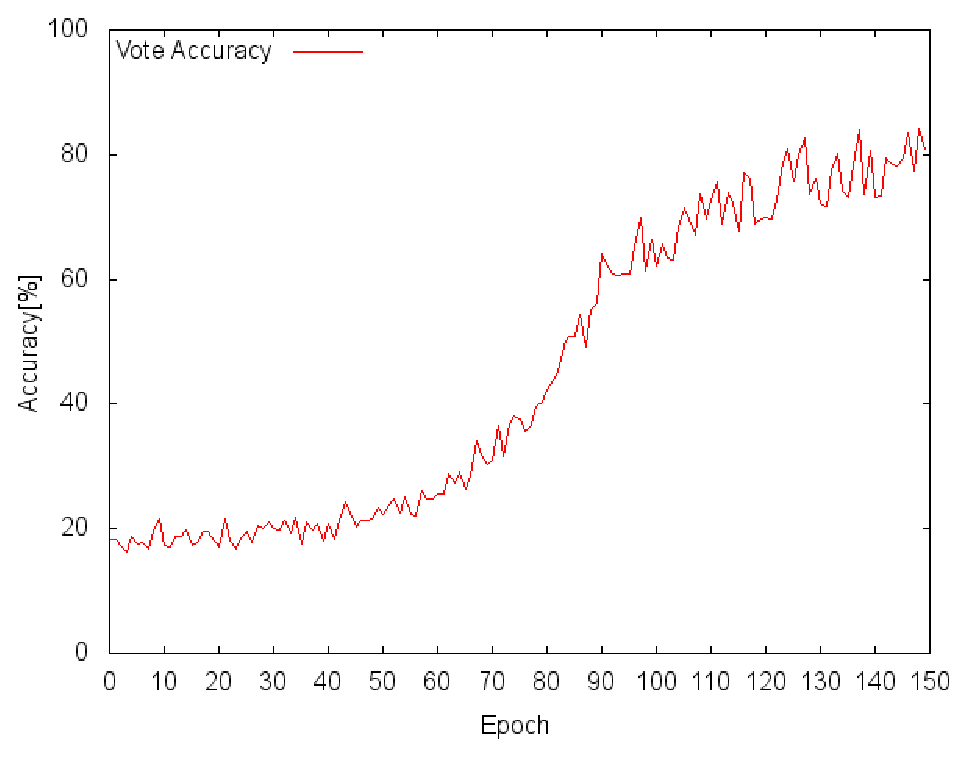
\includegraphics[width=85mm]{assets/accuracy.eps}
  \caption{Accuracy の推移}
  \label{fig:Accuracy}
\end{figure}

\section{実験結果}
表\ref{table:result}に実験結果を示す.図\ref{fig:Accuracy}に Accuracy の推移を示す.

\section{今後の課題}
今後の課題はうんぬんかんぬん〜

\bibliography{index}
\bibliographystyle{junsrt} %参考文献出力スタイル

\end{document}